
\subsection{Lepton Efficiencies}

We used the tag and probe method to study the lepton selection
efficiencies in the EPS and post-EPS datasets.
The post-EPS dataset was initially available in the PromptReco V5 processing,
which is known to contain ECAL calibration issues leading to large fake MET.
These studies were performed on the PromptReco V5 before the data was
reprocessed because the calibration issues are not expected to bias the
lepton efficiencies.

The electron and muon selections efficiencies in the two datasets
and compared in Tables \ref{tab:lp_eff_electrons} and \ref{tab:lp_eff_muons}
respectively.
Because we do not observe any significant change in the
lepton selection efficiencies, we perform the LP analysis
using the same data to simulation scale factors as the EPS analysis.

\begin{table}[!ht]
\begin{center}
\begin{tabular} {c|ccc}
\hline
          & $10<p_T<15$ & $15<p_T<20$ & $p_T>20$ \\
\hline
\multicolumn{4}{c} {Barrel ($|\eta|<1.479$)} \\ \hline
post-EPS       & $0.3955 \pm 0.0411$ & $0.5443 \pm 0.0090$ & $0.6808 \pm 0.0029$ \\
EPS            & $0.4064 \pm 0.0250$ & $0.5184 \pm 0.0076$ & $0.6891 \pm 0.0013$ \\ \hline
\multicolumn{4}{c} {Endcap ($|\eta|>1.479$)} \\ \hline
post-EPS       & $0.1935 \pm 0.0265$ & $0.3320 \pm 0.0218$ & $0.6808 \pm 0.0029$ \\
EPS            & $0.2079 \pm 0.0103$ & $0.3219 \pm 0.0101$ & $0.6891 \pm 0.0013$ \\
\hline
\end{tabular}
\caption{Comparison of the electron efficiencies in the EPS and post-EPS datasets.}
\label{tab:lp_eff_electrons}
\end{center}
\end{table}

\begin{table}[!ht]
\begin{center}
\begin{tabular} {c|ccc}
\hline
          & $10<p_T<15$ & $15<p_T<20$ & $p_T>20$ \\
\hline
\multicolumn{4}{c} {Barrel ($|\eta|<1.479$)} \\ \hline
post-EPS       & N/A                 & $0.7651 \pm 0.0188$ & $0.6808 \pm 0.0029$ \\
EPS            & $0.6620 \pm 0.0108$ & $0.7306 \pm 0.0047$ & $0.6891 \pm 0.0013$ \\ \hline
\multicolumn{4}{c} {Endcap ($|\eta|>1.479$)} \\ \hline
post-EPS       & N/A                 & $0.7543 \pm 0.0197$ & $0.9193 \pm 0.0010$ \\
EPS            & $0.7079 \pm 0.0110$ & $0.7235 \pm 0.0073$ & $0.9138 \pm 0.0008$ \\
\hline
\end{tabular}
\caption{Comparison of the muon efficiencies in the EPS and post-EPS datasets.
Note that the low $p_T$ efficiencies were not available for the post-EPS dataset at the time of writing
with the code used to produce these results.
An independent measurement of the data to simulation scale factors found
$0.91 \pm 0.01$ ($0.91 \pm 0.02$) for the EPS dataset and $0.95 \pm 0.02$ ($0.90 \pm 0.03$)
for the post-EPS dataset in the Barrel (Endcap) regions.}
\label{tab:lp_eff_muons}
\end{center}
\end{table}

%
%
%
\subsection{Pile-up Reweighting}
We perform a reweighting to take into account the difference
between the pile-up model used to generate the simulated data samples.
Because the expected pile-up distribution depends on the instantaneous
luminosity, we reweight to the target distribution that corresponds to
the dataset used.
The result of applying this procedure to the EPS, post-EPS and LP datasets
is shown in Figures \ref{subfig:lp_pureweight_eps}, \ref{subfig:lp_pureweight_posteps}
and \ref{subfig:lp_pureweight_lp} respectively.
In all cases we find good agreement between the data and the simulation
after reweighting.

\begin{figure}[!hbtp]
\centering
\subfigure[]{
\centering
\label{subfig:lp_pureweight_eps}
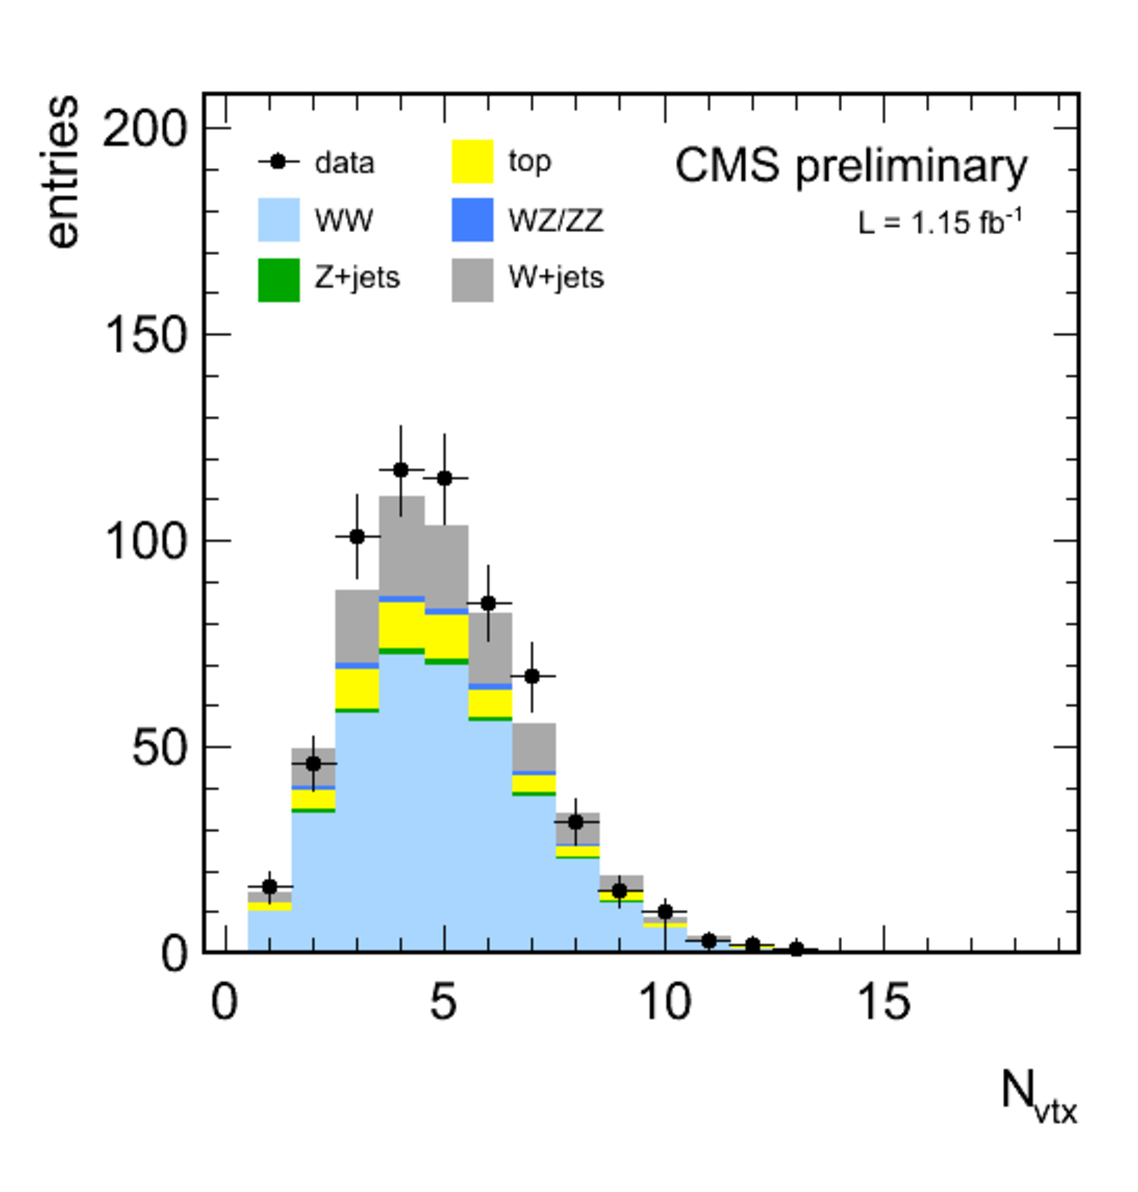
\includegraphics[width=.32\textwidth]{lp_figures/puReweight/histo_nvtx_ww0j_allhwwcuts_EPS.pdf}}
\subfigure[]{
\centering
\label{subfig:lp_pureweight_posteps}
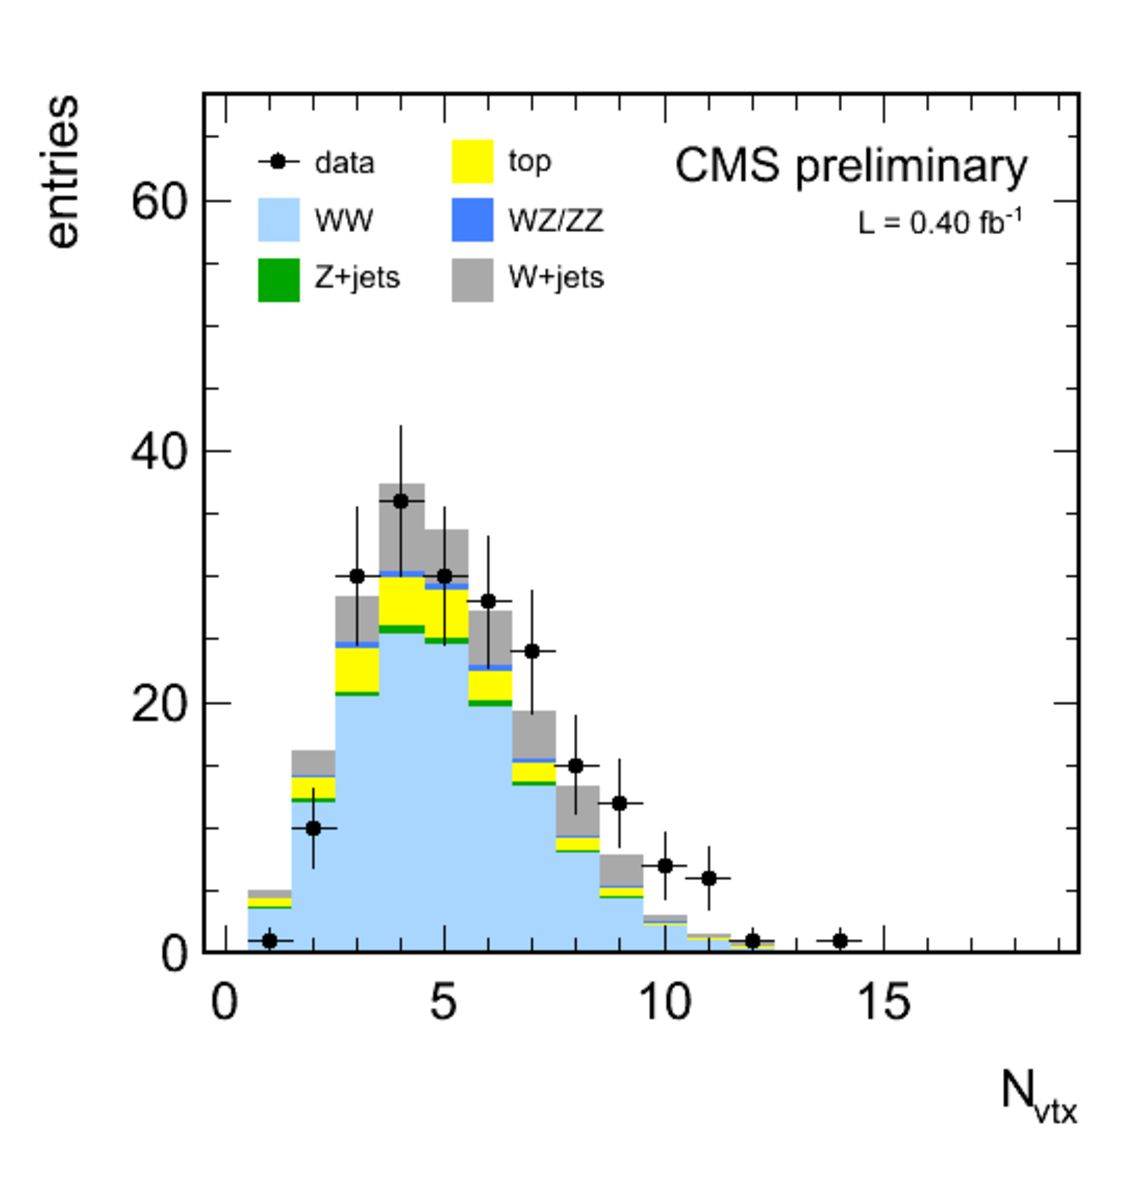
\includegraphics[width=.32\textwidth]{lp_figures/puReweight/histo_nvtx_ww0j_allhwwcuts_POSTEPS.pdf}}
\subfigure[]{
\centering
\label{subfig:lp_pureweight_lp}
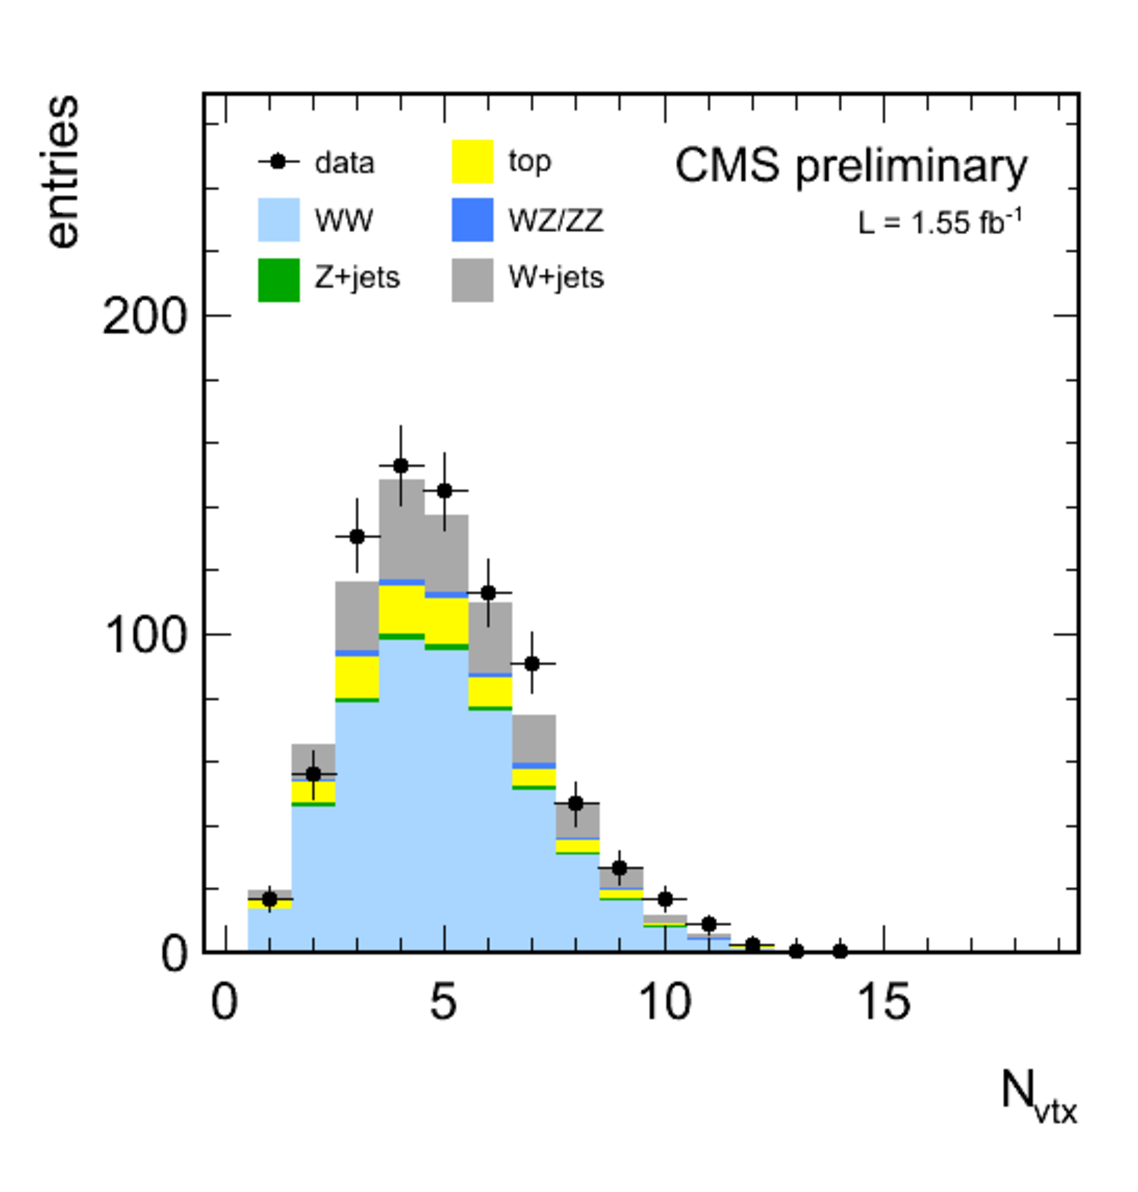
\includegraphics[width=.32\textwidth]{lp_figures/puReweight/histo_nvtx_ww0j_allhwwcuts.pdf}}
\caption{The number of reconstructed vertices in data and simulation
at the WW preselection level after pile-up reweighting
according to the expected pile-up multiplicity
\subref{subfig:lp_pureweight_eps} in the EPS dataset;
\subref{subfig:lp_pureweight_posteps} in the post-EPS dataset;
\subref{subfig:lp_pureweight_lp} in the LP dataset;
}
\label{fig:lp_ww0j_dilep}
\end{figure}



